\documentclass[main.tex]{subfiles}

\begin{document}
\subsection{GA with Clustering}
\begin{frame}{Encoding Scheme}
	\begin{itemize}
		\item Each individual is a 2-part list.
		\item The first N items is a permutation of sensor nodes.
		\item The next Y items are the selected relay nodes.
	\end{itemize}
	\begin{center}
		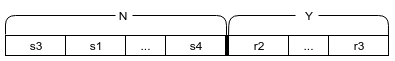
\includegraphics[scale=0.6]{WusnEncode.png}
	\end{center}
\end{frame}

\begin{frame}{Decoding}
	\begin{itemize}
		\item Each $N/Y$ block of SN is assigned to a corresponding RN.
	\end{itemize}
	\begin{center}
		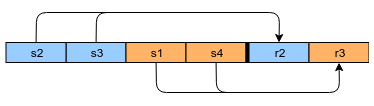
\includegraphics[scale=0.6]{WusnDecode.png}
	\end{center}
\end{frame}

\begin{frame}{Initialization}
	\begin{itemize}
		\item Use k-means to group all sensors into $Y$ clusters.
		\item For each cluster, assign an unselected relay that is closest to its centroid.
		\pause
		\item Problem: k-means cannot control how many sensors are in a cluster. $\rightarrow$ Likely break balance constraint.
		\pause
		\item Solution: Flatten the clusters and their relays and put them sequentially in the encoding. Some sensors may be assigned to a far away relay, but still acceptable for initial population.
		\item Each run of k-means can create a different individual (random initial centroids).
	\end{itemize}
\end{frame}

\begin{frame}{Crossover/Mutation}
	\begin{itemize}
		\item 2 operators for the sensor list and relay list.
		\pause
		\item {
			Crossover:
			\begin{itemize}
				\pause
				\item Sensor list: PMX operator, similar to TSP.
				\pause
				\item Relay list: 2-point crossover followed by normalization.
			\end{itemize}
		}
		\item {
			Mutation
			\begin{itemize}
				\item Sensor list: Swaps 2 random elements in the sensor list.
				\pause
				\item Relay list: Choose 2 random relays $r_{in} \in F$ and $r_{out} \in G$, where $G$ is the relay list and $r_{in} \neq r_{out}$.
				\item If $r_{in} \in G$, swap the positions of $r_{in}$ and $r_{out}$. 
				\item Otherwise, replace $r_{out}$ with $r_{in}$.
			\end{itemize}
		}
	\end{itemize}
\end{frame}

\begin{frame}{Selection}
	\begin{itemize}
		\item Fitness function: maximum loss value of the corresponding solution.
		\item Selection strategy: tournament selection. Select $n$ best individuals from a random subset of the population.
	\end{itemize}
\end{frame}

\end{document}
